%% ----------------------------------------------------------------
%% SETTINGS
%% ----------------------------------------------------------------
\documentclass[../informe.tex]{subfiles}

%% ----------------------------------------------------------------
%% BEGIN
%% ----------------------------------------------------------------
\begin{document}

%% ----------------------------------------------------------------
%% DOCUMENT
%% ----------------------------------------------------------------
En el campo de la electricidad, una de las mediciones más importantes es la de corriente eléctrica. Esta variable se extiende desde algunos picoamperes hasta miles de amperes. La selección de una técnica de sensado depende de requerimientos tales como la magnitud, precisión, ancho de banda, robustez, costo, aislación o tamaño. También se debe considerar la naturaleza de la corriente, es decir si es alterna o continua, y el impacto del dispositivo de medición en la operación del sistema. El valor de corriente puede ser mostrado en el mismo instrumento o convertido a formato digital para ser utilizado por un sistema de monitoreo o de control.

A continuación, se muestran algunos dispositivos de medición existentes.

%% ----------------------------------------------------------------
\subsection{Sondas de corriente}
%% ----------------------------------------------------------------
La medición de la corriente eléctrica puede ser clasificada dependiendo en el principio físico fundamental en el que se basa. Siguiendo esta distinción, se tienen los siguientes dispositivos.

  %% ----------------------------------------------------------------
  \subsubsection{Sondas de corriente basadas en la ley de Ohm}
  %% ----------------------------------------------------------------
  La ley de Ohm se refiere a la relación que hay entre la corriente que circula por una resistencia y la tensión que cae sobre ella. Este principio puede ser utilizado para medir corrientes, resultando en dispositivos baratos y confiables, dada la simplicidad de este enfoque.

  Los sensores de corriente que usan este método se los conoce como Resistencias de shunt. Permiten medir tanto corrientes alternas como continuas, presentan una buena respuesta a señales de alta frecuencia y se las puede encontrar en encapsulado de montado superficial. La mayor desventaja se encuentra cuando se trabaja con grandes valores de corriente, ya que al tratarse de una resistencia, la disipación de potencia aumenta cuadráticamente respecto de la misma.

  En la \autoref{fig:resistencia-shunt-foto} se puede observar un ejemplo de una resistencia de shunt comercial Vishay serie WSL3637.

      \begin{figure}[!htbp]
          \centering
          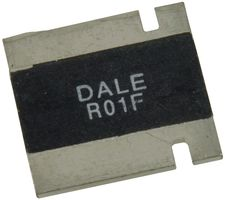
\includegraphics[scale=0.5]{images/resistencia-shunt-foto.jpg}
          \caption{Resistencia de shunt Vishay serie WSL3637}
          \label{fig:resistencia-shunt-foto}
      \end{figure}

  %% ----------------------------------------------------------------
  \subsubsection{Sondas de corriente basadas en el efecto Hall}
  %% ----------------------------------------------------------------
  El efecto Hall está basado en el principio físico de la fuerza Lorentz, que se refiere a la inducción de una fuerza electromotriz ante la presencia de un campo magnético. Este tipo de dispositivos proveen una precisión mucho menor que aquellos basados en la ley de Faraday, requiriendo además de compensación por temperatura y circuitería externa para ser utilizados. Permiten medir tanto corriente alterna como continua.

  Su uso principal en la industria es a modo de detección, utilizándose efectivamente como interruptores. También se los encuentra en multímetros.

  En la \autoref{fig:hall-foto} se puede ver un ejemplo de un sensor de efecto Hall comercial Honeywell serie GT1 utilizado para medir la velocidad de engranajes.

      \begin{figure}[!htbp]
          \centering
          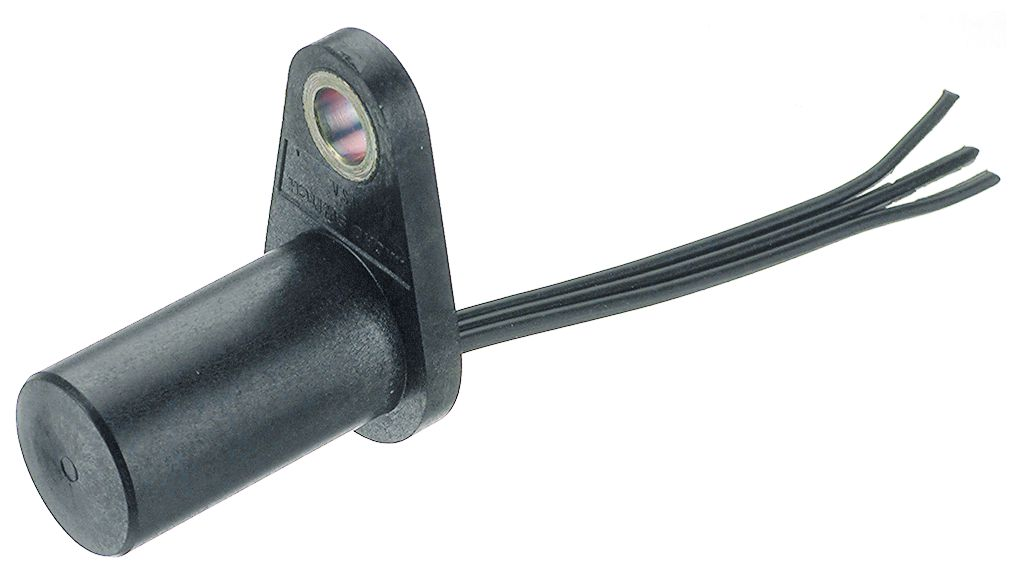
\includegraphics[scale=0.15]{images/hall-foto.jpg}
          \caption{Sensor de efecto Hall Honeywell serie GT1}
          \label{fig:hall-foto}
      \end{figure}

  %% ----------------------------------------------------------------
  \subsubsection{Sondas de corriente basadas en la ley de Faraday}
  %% ----------------------------------------------------------------
  La ley de Faraday se refiere a la inducción de fuerza electromotriz que se produce ante cambios en el flujo magnético. Los transformadores de corriente y las bobinas de Rogowski utilizan este principio. Estos sensores proveen una aislación eléctrica intrínseca al método de medición entre la señal de salida y la corriente medida, logrando así una mayor seguridad. Debido a que las corrientes continuas no producen un campo magnético variable, este tipo de dispositivos está limitado a su uso con corrientes alternas.

    %% ----------------------------------------------------------------
    \paragraph{Transformadores de corriente}
    %% ----------------------------------------------------------------
    Estos instrumentos permite convertir la alta corriente presente en un circuito en un valor mucho menor. Es común su utilización en sistemas de alta corriente alterna. Una desventaja de los mismos es que una magnitud elevada de corriente o una componente continua de la misma puede saturar su núcleo de hierro, corrompiendo así la medición. Debido a su material de construcción, resulta en un dispositivo muy pesado y al ser cerrado, es necesario interrumpir el circuito a medir para poder utilizarlo.

    En la \autoref{fig:trafo-corriente} se puede observar un ejemplo de un transformador de corriente comercial Arteche IRH-3.

        \begin{figure}[!htbp]
            \centering
            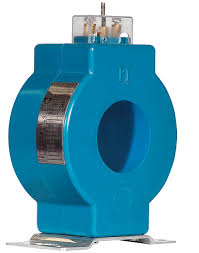
\includegraphics[scale=0.5]{images/trafo-corriente.jpg}
            \caption{Transformador de corriente Arteche IRH-3}
            \label{fig:trafo-corriente}
        \end{figure}

    %% ----------------------------------------------------------------
    \paragraph{Bobinas de Rogowski}
    %% ----------------------------------------------------------------
    Estos dispositivos de medición, similares a los anteriores, generan una tensión entre sus bornes la cual debe ser integrada para poder obtener un valor proporcional a la corriente presente en el circuito. Esto presenta una desventaja, ya que el circuito de integración debe ser alimentado. Sin embargo, debido a que utilizan un núcleo de aire presentan varias ventajas: no sufren de saturación magnética, permitiendo su uso en un amplio rango de frecuencias; no es necesario interrumpir el circuito para realizar la medición; y tienen bajos costos de construcción, pudiendo ser diseñados para ser flexibles y de bajo peso.

    En la \autoref{fig:rogowski-foto} se puede ver un ejemplo de una bobina de Rogowski comercial Fluke i3000.

        \begin{figure}[!htbp]
            \centering
            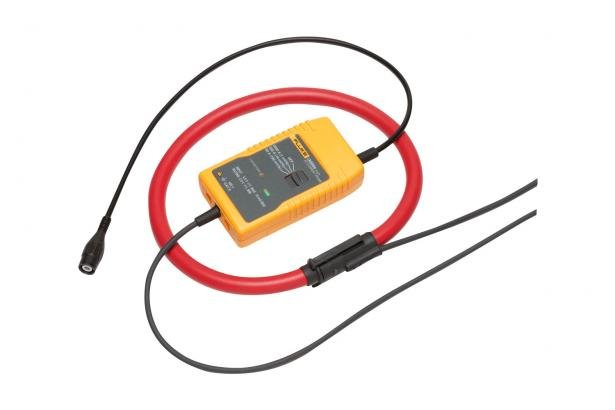
\includegraphics[scale=0.6]{images/rogowski-foto.jpg}
            \caption{Bobina de Rogowski Fluke i3000}
            \label{fig:rogowski-foto}
        \end{figure}

%% ----------------------------------------------------------------
\subsection{Uso y aplicación}
%% ----------------------------------------------------------------
La sonda elegida para calibrar y caracterizar por este instrumento es la bobina de Rogowski. Este tipo de sensores son de particular interés para el Laboratorio de Instrumentación y Control, perteneciente al INCyTE, del cual surge la idea original de este proyecto. Esto es así ya que presentan características relevantes al trabajo realizado allí:

    \begin{itemize}
        \item Simples de construir, lo cual permite crear un prototipo con el material disponible en el Laboratorio.
        \item Estructura flexible, haciéndolos fáciles de instalar o remover.
        \item Bajo costo, necesario dado que se necesitan al menos cuatro por equipo trifásico.
    \end{itemize}

Estos dispositivos son utilizados en el estudio y desarrollo de medidores de calidad del suministro eléctrico por el Laboratorio. Es de esta forma que surge la necesidad de tener un instrumento de banco capaz de calibrarlas y caracterizarlas.

Se exploraron alternativas comerciales tales como el Fluke 5500A/COIL y el Fluke 52120A vistos en la \autoref{fig:fluke-5500a-foto} y \autoref{fig:fluke-52120a-foto} respectivamente. Sin embargo, la selección manual de parámetros de la señal generada hacía que las sesiones de calibración y caracterización sean largas y engorrosas.

    \begin{figure}[!htbp]
        \centering
        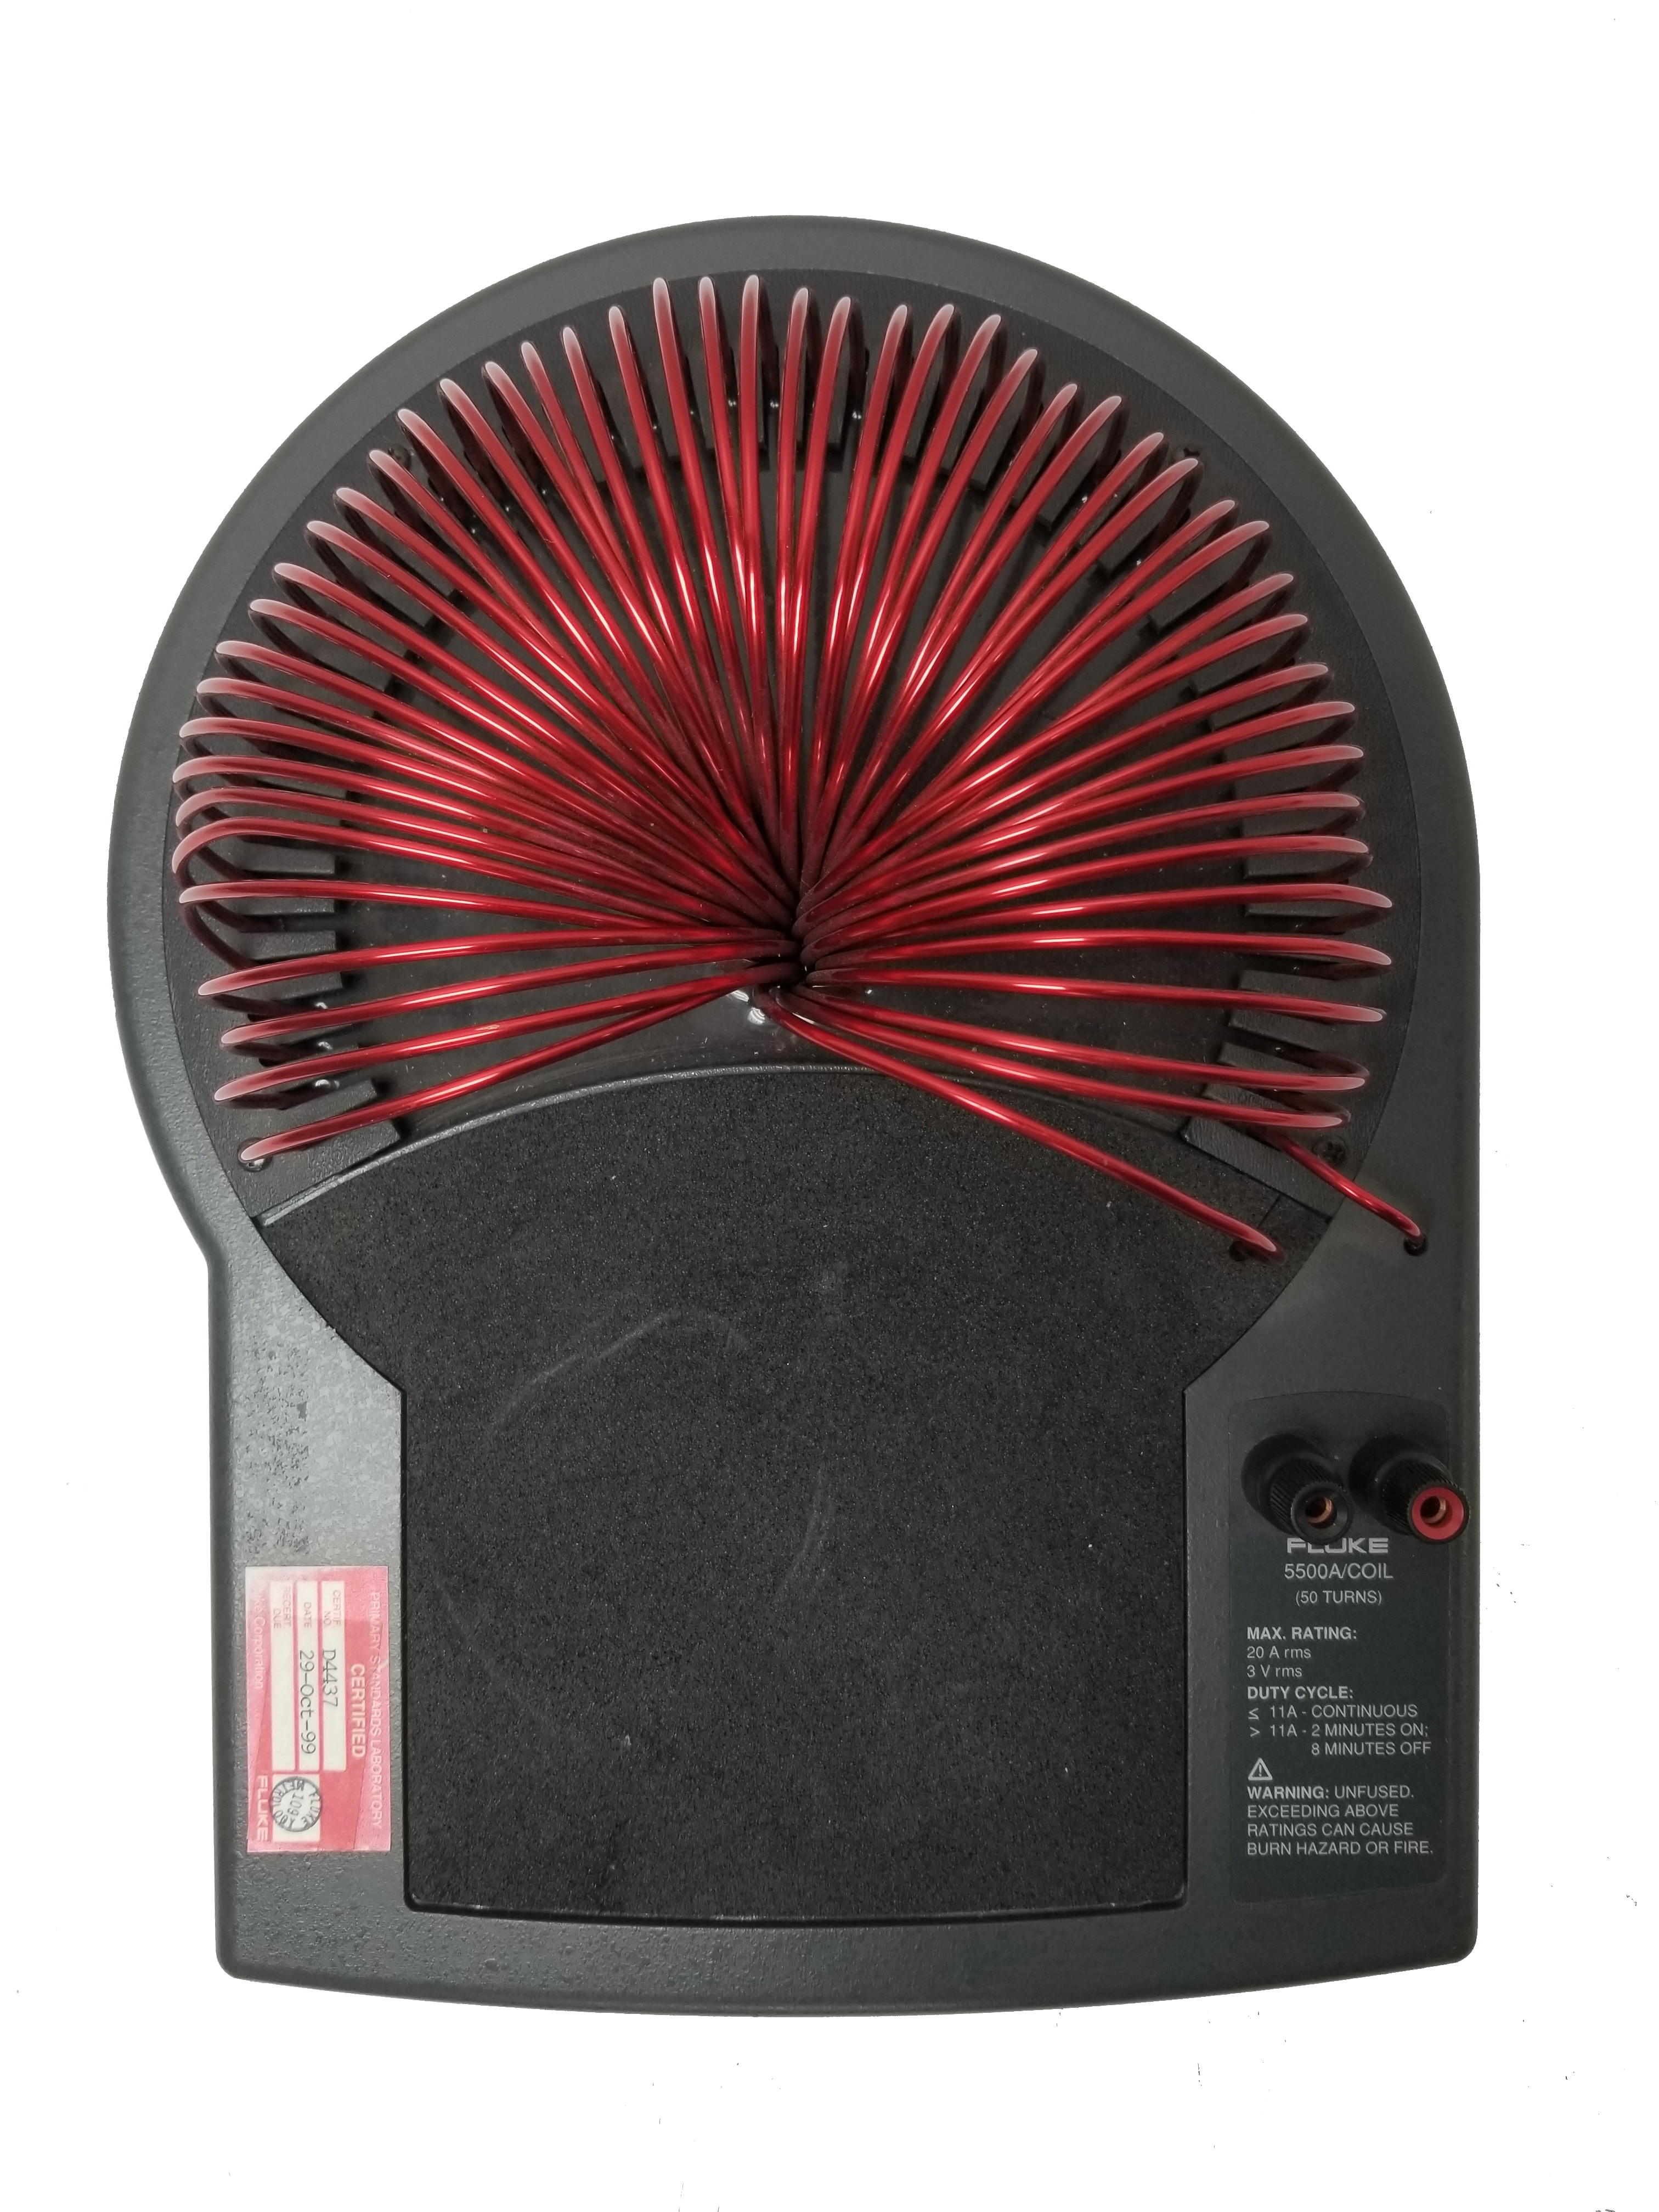
\includegraphics[scale=0.07]{images/fluke-5500a-foto.jpg}
        \caption{Fluke 5500A/COIL}
        \label{fig:fluke-5500a-foto}
    \end{figure}

    \begin{figure}[!htbp]
        \centering
        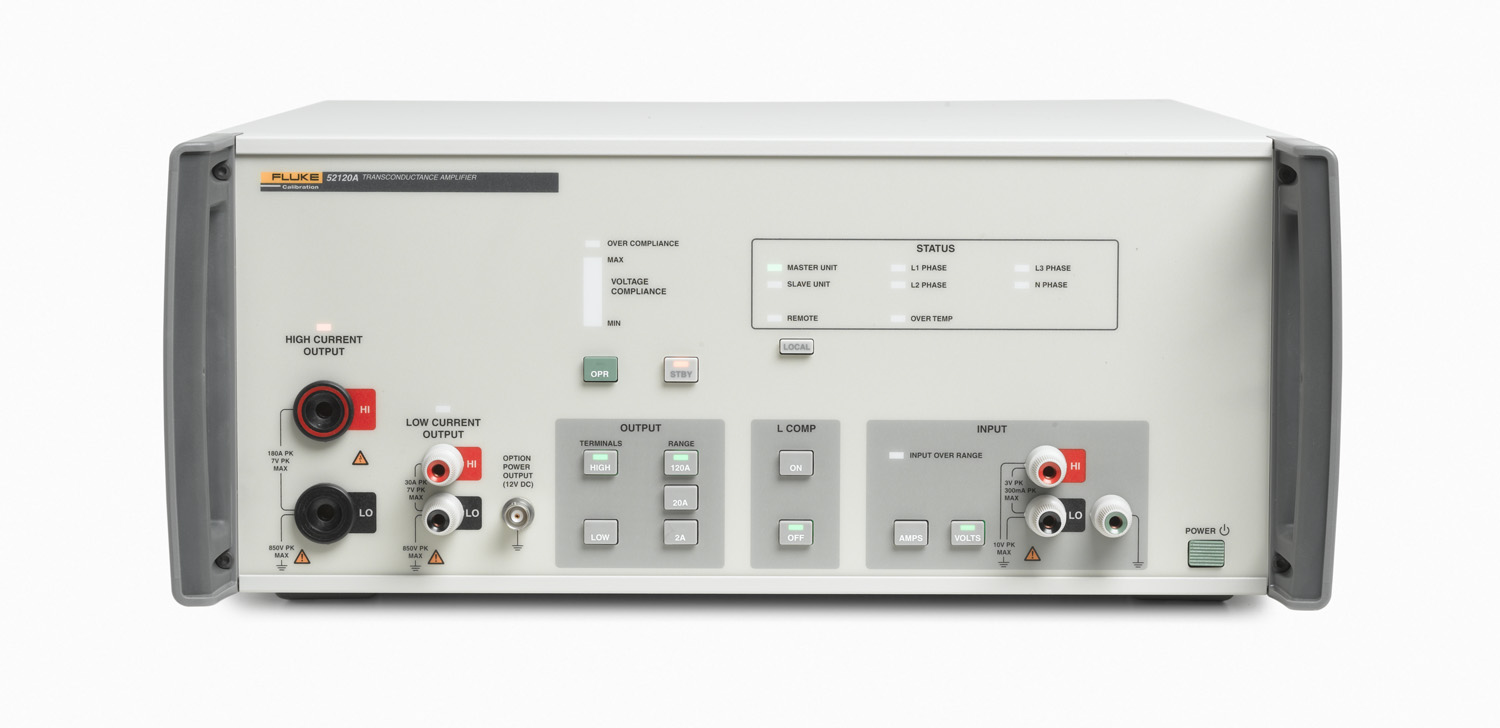
\includegraphics[scale=0.7]{images/fluke-52120a-foto.jpg}
        \caption{Fluke 52120A}
        \label{fig:fluke-52120a-foto}
    \end{figure}

De esta forma se decide proceder con la construcción de un instrumento de banco capaz de automatizar estos ensayos y añadir valor agregado a los reportes generados por el Laboratorio.

%% ----------------------------------------------------------------
%% END
%% ----------------------------------------------------------------
\end{document}